% !TEX TS-program = XeLaTeX
% use the following command:
% all document files must be coded in UTF-8
\documentclass[portuguese]{textolivre}
% build HTML with: make4ht -e build.lua -c textolivre.cfg -x -u article "fn-in,svg,pic-align"

\journalname{Texto Livre}
\thevolume{15}
%\thenumber{1} % old template
\theyear{2022}
\receiveddate{\DTMdisplaydate{2021}{12}{20}{-1}} % YYYY MM DD
\accepteddate{\DTMdisplaydate{2022}{3}{17}{-1}}
\publisheddate{\DTMdisplaydate{2022}{5}{14}{-1}}
\corrauthor{Manoel Francisco Guaranha}
\articledoi{10.35699/1983-3652.2022.37569}
%\articleid{NNNN} % if the article ID is not the last 5 numbers of its DOI, provide it using \articleid{} commmand 
% list of available sesscions in the journal: articles, dossier, reports, essays, reviews, interviews, editorial
\articlesessionname{articles}
\runningauthor{Pacheco e Guaranha} 
%\editorname{Leonardo Araújo} % old template
\sectioneditorname{Daniervelin Pereira}
\layouteditorname{Leonado Araújo}

\title{\textit{Parser} sintático para o português brasileiro: desafios e soluções}
\othertitle{Syntactic parser for Brazilian Portuguese: challenges and solutions}
% if there is a third language title, add here:
%\othertitle{Artikelvorlage zur Einreichung beim Texto Livre Journal}

\author[1]{Willian Emerson Afonso Pacheco \orcid{0000-0003-0395-0303} \thanks{Email: \url{willian.pacheco@fatec.sp.gov.br}}}
\author[1,2]{Manoel Francisco Guaranha~\orcid{0000-0002-8676-601X}~\thanks{Email: \url{manoel.guaranha@gmail.com}}}
\affil[1]{Faculdade de Tecnologia do Estado de São Paulo, Câmara de Ensino, Extensão e Pesquisa da FATEC Ipiranga, São Paulo, SP, Brasil.}
\affil[2]{Universidade Santo Amaro, Programa de Mestrado em Ciências Humanas, São Paulo, SP, Brasil.}

\addbibresource{article.bib}
% use biber instead of bibtex
% $ biber article

% used to create dummy text for the template file
\definecolor{dark-gray}{gray}{0.35} % color used to display dummy texts
\usepackage{lipsum}
\SetLipsumParListSurrounders{\colorlet{oldcolor}{.}\color{dark-gray}}{\color{oldcolor}}

% used here only to provide the XeLaTeX and BibTeX logos
\usepackage{hologo}

% if you use multirows in a table, include the multirow package
\usepackage{multirow}

% provides sidewaysfigure environment
\usepackage{rotating}

% CUSTOM EPIGRAPH - BEGIN 
%%% https://tex.stackexchange.com/questions/193178/specific-epigraph-style
\usepackage{epigraph}
\renewcommand\textflush{flushright}
\makeatletter
\newlength\epitextskip
\pretocmd{\@epitext}{\em}{}{}
\apptocmd{\@epitext}{\em}{}{}
\patchcmd{\epigraph}{\@epitext{#1}\\}{\@epitext{#1}\\[\epitextskip]}{}{}
\makeatother
\setlength\epigraphrule{0pt}
\setlength\epitextskip{0.5ex}
\setlength\epigraphwidth{.7\textwidth}
% CUSTOM EPIGRAPH - END

% LANGUAGE - BEGIN
% ARABIC
% for languages that use special fonts, you must provide the typeface that will be used
% \setotherlanguage{arabic}
% \newfontfamily\arabicfont[Script=Arabic]{Amiri}
% \newfontfamily\arabicfontsf[Script=Arabic]{Amiri}
% \newfontfamily\arabicfonttt[Script=Arabic]{Amiri}
%
% in the article, to add arabic text use: \textlang{arabic}{ ... }
%
% RUSSIAN
% for russian text we also need to define fonts with support for Cyrillic script
% \usepackage{fontspec}
% \setotherlanguage{russian}
% \newfontfamily\cyrillicfont{Times New Roman}
% \newfontfamily\cyrillicfontsf{Times New Roman}[Script=Cyrillic]
% \newfontfamily\cyrillicfonttt{Times New Roman}[Script=Cyrillic]
%
% in the text use \begin{russian} ... \end{russian}
% LANGUAGE - END

% EMOJIS - BEGIN
% to use emoticons in your manuscript
% https://stackoverflow.com/questions/190145/how-to-insert-emoticons-in-latex/57076064
% using font Symbola, which has full support
% the font may be downloaded at:
% https://dn-works.com/ufas/
% add to preamble:
% \newfontfamily\Symbola{Symbola}
% in the text use:
% {\Symbola }
% EMOJIS - END

% LABEL REFERENCE TO DESCRIPTIVE LIST - BEGIN
% reference itens in a descriptive list using their labels instead of numbers
% insert the code below in the preambule:
%\makeatletter
%\let\orgdescriptionlabel\descriptionlabel
%\renewcommand*{\descriptionlabel}[1]{%
%  \let\orglabel\label
%  \let\label\@gobble
%  \phantomsection
%  \edef\@currentlabel{#1\unskip}%
%  \let\label\orglabel
%  \orgdescriptionlabel{#1}%
%}
%\makeatother
%
% in your document, use as illustraded here:
%\begin{description}
%  \item[first\label{itm1}] this is only an example;
%  % ...  add more items
%\end{description}
% LABEL REFERENCE TO DESCRIPTIVE LIST - END


% add line numbers for submission
%\usepackage{lineno}
%\linenumbers

\usepackage[linesnumbered,lined,commentsnumbered]{algorithm2e}

\begin{document}
\maketitle

\begin{polyabstract}
\begin{abstract}
Este artigo tem como objetivo apresentar o Parser Sintático para o Português Brasileiro – \textit{Parsero}, desenvolvido a partir da Gramática Gerativa \cite{chomsky_estruturas_2015}, aperfeiçoada pela Teoria X-Barra \cite{chomsky__2014}. Para tanto, foram utilizadas as regras desenvolvidas especialmente para o Português Brasileiro por \textcite{othero_gramatica_2009} e adaptadas pelo nosso projeto para atender às necessidades de nosso Parser. A pesquisa utilizou como coleção lexical, para povoar um Banco de Dados \textit{Structured Query Language} (SQL), o recurso \textit{Dicionário de Palavras Simples Flexionadas para o Português Brasileiro} (DELAF\_PB), disponibilizado pelo Projeto Unitex-PB, desenvolvido pelo Núcleo Interinstitucional de Linguística Computacional (NILC) e pelo Instituto de Ciências Matemáticas e de Computação (ICMC). Esse recurso, por sua vez, foi construído com base no formalismo francês – \textit{Dictionnarie Electronique du LADL} (DELA) \cite{muniz_construcao_2004}. Como resultado, disponibilizamos a Base de Dados SQL com 1.193.295 unidades léxicas classificadas, o endereço com o código aberto do \textit{Parsero} e um \textit{link} para execução do aplicativo. Para desenvolver o Processador de Linguagem Natural (PLN), colocamos em prática estudos interdisciplinares em ciências da linguagem e ciências da computação, práticas necessárias para o desenvolvimento de programas inteligentes que consigam interagir com escritores e falantes do Português Brasileiro. 

\keywords{Linguística computacional \sep Processamento de Linguagem Natural \sep Gramática gerativa \sep Parser sintático \sep Português brasileiro}
\end{abstract}

\begin{english}
\begin{abstract}
This article aims to present the Syntactic Parser for Brazilian Portuguese – Parsero –, developed from the Generative Grammar \cite{chomsky_estruturas_2015} improved by the X-Barra Theory \cite{chomsky__2014}. Therefore, the rules developed by \textcite{othero_gramatica_2009} especially for Brazilian Portuguese were used and adapted by our project to meet the needs of our Parser. The research used as lexical collection, to populate a \textit{Structured Query Language} (SQL) Database, the resource \textit{Dictionary of Simple Inflected Words for Brazilian Portuguese} (DELAF\_PB), which was made available available by the Unitex-PB Project, developed by Núcleo Interinstitucional de Linguística Computacional (NILC) and by Instituto de Ciências Matemáticas e de Computação (ICMC). This resource, in turn, was built based on the French formalism – \textit{Dictionnarie Electronique du LADL} (DELA) \cite{muniz_construcao_2004}. As a result of our project, we have made available to researchers interested in the topic the SQL Database with 1,193,295 classified lexical units, the address with the open source of \textit{Parsero} and a link to run the application. Throughout the development of the Natural Language Processor (NLP), we had to put into practice interdisciplinary studies from language sciences and computer sciences, a necessary practice for the development of intelligent programs that can interact with writers or Brazilian Portuguese speakers.

\keywords{Computational linguistics \sep Natural Language Processing \sep Generative Grammar \sep Syntactic parser \sep Brazilian Portuguese}
\end{abstract}
\end{english}
% if there is another abstract, insert it here using the same scheme
\end{polyabstract}

\section{Considerações iniciais}\label{sec-intro}
Um dos problemas mais instigantes na área de processamento computacional é o de construção de \textit{Parsers} sintáticos, sistemas que, dada uma sentença ou mais, produzem suas árvores sintáticas. Os desafios que se colocam na construção desses leitores eletrônicos compreendem as seguintes etapas: a construção e manutenção de um conjunto de itens lexicais organizados de modo a facilitar o processamento, já que o conjunto de palavras de uma língua é extenso e, pode-se dizer, aberto a novos termos que surgem a partir dos diferentes usos; a construção de algoritmos morfossintáticos, capazes de rotular os itens lexicais segundo sua função, uma vez que o valor posicional de cada unidade ou locução varia de acordo com a posição que ocupa nos enunciados; a construção de algoritmos capazes de agrupar os itens lexicais em sintagmas, atribuindo-lhes as funções sintáticas e validando-os segundo as regras de combinação estabelecidas pela gramática. Em cursos tecnológicos de Análise e Desenvolvimento de Sistemas, a investigação de processos de construção de \textit{Parsers} sintáticos constitui uma tarefa interdisciplinar que oferece oportunidade de aprendizagem aos pesquisadores, tanto aos que se dedicam ao estudo das estruturas da língua, português falado no Brasil, no nosso caso, quanto àqueles que investigam estruturas de dados e de linguagens de programação que sejam adequadas para o Processamento de Linguagem Natural (PLN) que, diferentemente do processamento de números, sujeito às regras rígidas da Matemática, requerem processos mais complexos de tratamento. Sendo assim, o projeto descrito neste artigo disponibilizou, para pesquisadores interessados no tema, o aplicativo de PLN \textit{Parsero}, e o Banco de Dados com o léxico do Português Brasileiro.

Este artigo pretende apresentar, portanto, o processo de elaboração do Parser Sintático para o Português Brasileiro - \textit{Parsero}, que analisa sentenças escritas, bem como seus resultados, obtidos por meio de uma pesquisa realizada no Curso Superior de \textit{Tecnologia em Análise e Desenvolvimento de Sistemas} da Faculdade de Tecnologia do Estado de São Paulo (FATEC), no âmbito da \textit{Câmara de Ensino, Pesquisa e Extensão} CEPE/Fatec Ipiranga). Para tanto, foram utilizados os conceitos da Gramática Gerativa de \textcite{chomsky__2014,chomsky_estruturas_2015} (originais publicados em 1957 e 2012, respectivamente), com adaptações propostas por \textcite{othero_gramatica_2009} para atender às especificidades do Português Brasileiro e, além disso, com adaptações que foram necessárias para atender às especificidades deste projeto. A pesquisa utilizou como recurso para construção de um banco de dados do léxico o \textit{Dicionário de Palavras Simples Flexionadas para o Português Brasileiro} (DELAF\_PB), arquivo com aproximadamente 880.000 palavras. Esse recurso, cuja documentação detalhada pode ser encontrada em \textcite{muniz_construcao_2004}, foi disponibilizado pelo Projeto Unitex-PB, desenvolvido pelo \textit{Núcleo Interinstitucional de Linguística Computacional} (NILC) e pelo \textit{Instituto de Ciências Matemáticas e de Computação} (ICMC) e foi construído com base no formalismo francês \textit{Dictionnarie Electronique du LADL} (DELA) \cite{muniz_construcao_2004}.  

A pesquisa desenvolveu, documentou e disponibilizou em repositórios virtuais três recursos linguístico-computacionais para o Português Brasileiro: o Banco de Dados SQL (\textit{Structured Query Language}) ParseroDB \cite{pacheco_banco_2021, pacheco_parser-api_2021}; o código aberto do processador sintático \textit{Parsero} \cite{pacheco_parser-api_2021}; e uma interface visual para execução do \textit{software} \cite{noauthor_parsero:_2021}. Espera-se que esses recursos possam ser utilizados e, eventualmente, aperfeiçoados por pesquisadores que se interessem em avançar nos trabalhos de desenvolvimento de sistemas na área de Processamento de Linguagem Natural para o Português Brasileiro. 

Para dar conta de nosso objetivo de apresentar o processo de construção do \textit{Parsero} e seus resultados, este artigo será desenvolvido em três seções, além das considerações iniciais e finais, numeradas como \cref{sec-intro} e \cref{sec-modelo}. Na \cref{sec-conduta}, discutiremos aspectos gerais da Gramática Gerativa proposta por \textcite{chomsky_estruturas_2015} e aperfeiçoada pela Teoria X-Barra, conforme afirma o próprio \textcite[p. 392]{chomsky__2014}. Na \cref{sec-fmt-manuscrito}, apresentaremos o Banco de Dados SQL que serviu de corpus para o nosso Processador de Linguagem Natural, detalhando o processo de construção desse recurso. Na \cref{sec-formato}, apresentaremos as características de nosso \textit{Parser}, o \textit{Parsero}, e as regras da Gramática Gerativa adaptadas para o Português Brasileiro por \textcite{othero_gramatica_2009}\footnote{Optamos por utilizar em nosso projeto os termos em português “Sintagma Verbal” (SV), “Sintagma Nominal” (SN), e assim por diante, em lugar de “\textit{Verb Phrase}” (VP), “\textit{Noun Phrase}” (NP) etc., termos em inglês, que foram utilizados por \textcite{othero_gramatica_2009}.}, que foram utilizadas no algoritmo, justificando, ainda, algumas adaptações que fizemos para atender às nossas necessidades. Nessa última seção também apresentaremos exemplos de sentenças processadas pelo aplicativo.

\section{Gramática Gerativa: potencialidades para o Processamento de Linguagem Natural (PLN)}\label{sec-conduta}
Consideramos a língua “um conjunto (finito ou infinito) de sentenças, cada sentença sendo finita em extensão e construída a partir de um conjunto finito de elementos” \cite[p. 18]{chomsky_estruturas_2015}. Essa concepção possibilita-nos estabelecer regras que possam separar sentenças gramaticais, que são reconhecidas como tal em uma língua, que parecem “aceitáveis a um falante nativo” \cite[p. 18]{chomsky_estruturas_2015}, das sentenças agramaticais, as que não são aceitáveis. Assim, podemos entender a gramática de uma língua como um “mecanismo que gera todas as sequências gramaticais” \cite[p. 18]{chomsky_estruturas_2015} dessa língua.  Dado que “[q]ualquer gramática de uma língua irá \textit{projetar} o \textit{corpus} de enunciados observados, finito e mais ou menos acidental, em um conjunto (presumivelmente infinito) de enunciados gramaticais” \cite[p. 19, grifos do autor]{chomsky_estruturas_2015}, pode-se dizer que “uma gramática reflete o comportamento do falante, que, baseado em uma experiência finita e acidental com a língua, pode produzir ou compreender um número indefinido de novas sentenças.” \cite[p. 19]{chomsky_estruturas_2015}.

Quando falamos em sequências gramaticais de uma língua, falamos da perspectiva morfossintática, e não semântica. Podemos parafrasear Chomsky construindo sentenças como (1) “infinitos pássaros dormem em espelhos de açúcar” e (2) “pássaros os acima voam cabeças das dos homens”. No caso de (1), ainda que a sequência não seja “dotada de sentido” ou “significativa” em um contexto não literário, pode ser considerada gramatical do ponto de vista da organização dos seus constituintes. No caso de (2), ainda que possamos, com alguma dificuldade, reorganizar os constituintes e compreender o significado do conjunto, temos uma estrutura não aceitável como está, agramatical portanto. 

Chegamos, portanto, a um conceito geral de Gramática, em que cada sentença pode ser decomposta em unidades constituintes denominadas sintagmas. Essas unidades têm como núcleo as categorias gramaticais da língua e se relacionam entre si em uma estrutura de sentido que pode ser expressa em formato que se assemelha a uma árvore (\Cref{fig1}). Essas estruturas formais permitem que possamos estabelecer regras gerais para uma língua.

\begin{figure}[htbp]
 \centering
 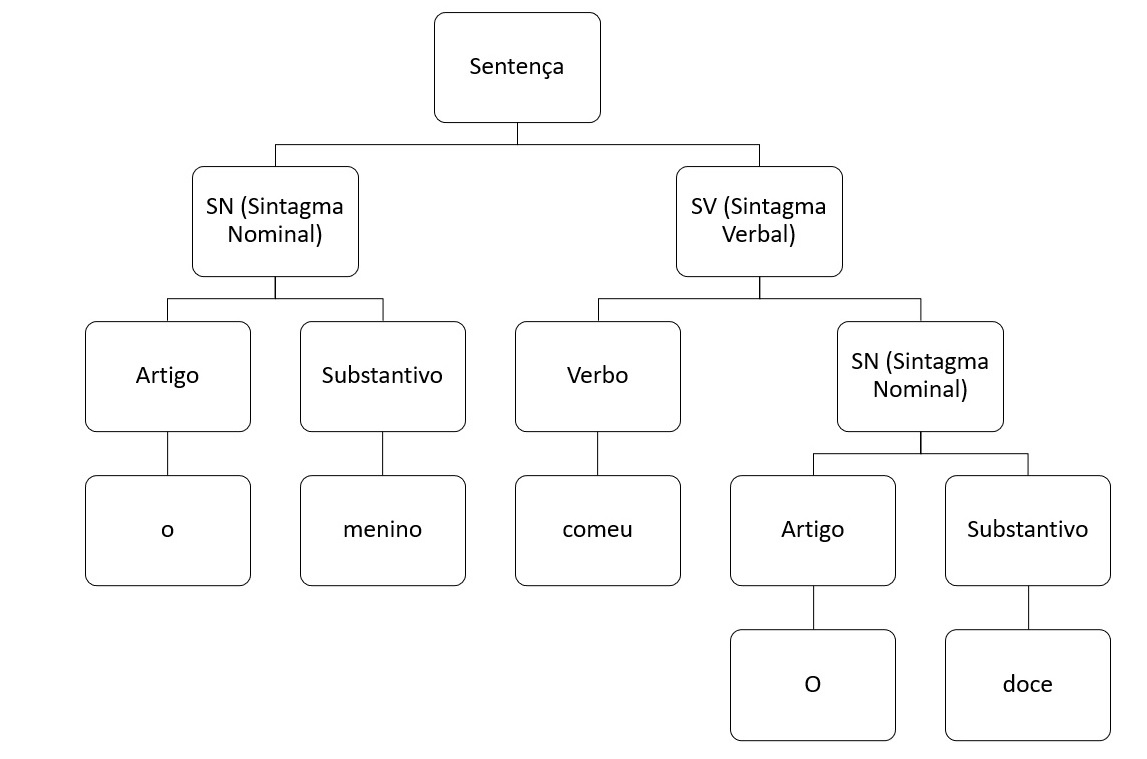
\includegraphics[width=\textwidth]{Fig1.png}
 \caption{Diagrama arbóreo de (3) O menino comeu o doce.}
 \label{fig1}
 \source{Autoria própria.}
\end{figure}

Para uma descrição mais detalhada dessa teoria, remetemos o leitor a \textcite{chomsky_estruturas_2015} e, para um estudo dessas estruturas no português, para \textcite{souza_e_silva_linguistica_2011,othero_gramatica_2009}. O exemplo de decomposição e de sentença que apresentaremos a seguir foi adaptado de \textcite[p. 38-39]{chomsky_estruturas_2015}. Dada a sentença (3) “O menino comeu o doce”, percebemos que as palavras não são agrupadas de modo aleatório, mas seguem regras de agrupamento que podem ser representadas do seguinte modo:

\begin{enumerate}[topsep=10pt]
    \item Sentença → SN (Sintagma nominal) + SV (Sintagma verbal)
    \item SN → Artigo + Nome
    \item SV → Verbo + SN
    \item Artigo → o, a, os, as...
    \item Nome → menino, menina, meninos, meninas, bolo, bolos, doce, doces...
    \item Verbo → comeu, comeram, pegou, pegaram, comprou, compraram...
\end{enumerate}

Cada regra deve ser interpretada na forma X → Y como a instrução “reescreva X como Y”, de modo que teríamos como gerar, por substituição, sentenças como (4) “O menino comeu o bolo”; (5) “A menina comprou o doce”; (6) “Os meninos pegaram os bolos” e assim por diante. Poderíamos, igualmente, gerar sentenças como (7) “O bolo comeu o doce”; (8) “Os doces comeram as meninas”, entre outras que seriam gramaticalmente aceitáveis, embora não o fossem semanticamente, pelo menos em contextos não literários. Podemos, ainda, determinar regras que regulam a organização dos termos no interior dos sintagmas em uma língua como o Português: artigos femininos no plural só podem estar ligados a substantivos femininos no plural, por exemplo. Também podemos determinar regras que regulam o relacionamento entre os sintagmas: caso o Sintagma Nominal fosse composto por um artigo e um substantivo no plural, o verbo teria de estar conjugado na terceira pessoa do plural, e assim por diante. O diagrama da \Cref{fig1} seria um modo de representar uma gramática que analisa os constituintes a partir de um conjunto de regras que especificamos. Uma sequência de palavras é um constituinte se pudermos ligá-la “a um único ponto de origem” ao qual atribuímos um rótulo. Percebe-se pelo diagrama arbóreo da \Cref{fig1} que o Sintagma Nominal aparece no nível abaixo da Sentença, ao lado do Sintagma Verbal, e que também aparece como componente do Sintagma Verbal. No primeiro caso, ele desempenha a função de sujeito: “O menino”; no segundo, de objeto direto: “o doce”.

Com a finalidade de atender ao Português Brasileiro, as regras originais propostas por \textcite{chomsky_estruturas_2015} precisam ser adaptadas, ainda que não alteradas em sua essência. Um excelente trabalho nesse aspecto foi desenvolvido por \textcite{othero_gramatica_2009}. Trata-se de uma pesquisa detalhada e consistente que serviu de base para a construção de nosso algoritmo. Na seção seguinte, vamos apresentar a Base de Dados que é utilizada por nosso \textit{Parser} e, na \Cref{sec-formato}, as características técnicas e de processamento segundo as regras estudadas em \textcite[p. 142]{othero_gramatica_2009}, com algumas adaptações e justificativas.

\section{Modelagem e construção do Banco de Dados do Parser \textit{Parsero}}\label{sec-fmt-manuscrito}
Para o Processamento de Linguagem Natural, o primeiro problema é ter um léxico categorizado e atualizado, trabalho que requer pesquisa criteriosa e custosa. Encontramos esse material disponível no banco de dados DELAF\_PB \cite{muniz_construcao_2004,muniz_delaf-pb:_2015}. O DELAF\_PB é um arquivo em formato “dic” que contém 9.072.146 de linhas com palavras simples e flexionadas, conforme o padrão: palavra, canônica. Classe+traços: flexão. Cada linha é uma entrada de texto terminada com um caractere de quebra de linha (\textbackslash n) e composta por até cinco campos delimitados por pontuação de acordo com o formato do \textit{Dictionnarie Electronique du LADL} (DELA) \cite[p. 17]{muniz_construcao_2004}.

Nesse formato, conforme o exemplo “fundamental,fundamental.ADJ+Pd:ms:fs”, uma vírgula (“,”) foi utilizada para separar as duas formas de cada palavra, a flexionada e a canônica, não flexionada. Para substantivos e adjetivos, a forma canônica está atribuída ao gênero masculino, quando não se trata de palavra de dois gêneros, e, para verbos, está no infinitivo. Um ponto (“.”) à frente de uma palavra precede a indicação de uma categoria correspondente às classes gramaticais: substantivos, adjetivos, artigos, preposições, conjunções, numerais, pronomes, verbos, advérbios e interjeições. Também há entradas para prefixos, siglas e abreviaturas. Cada verbete pode estar categorizado em mais de uma classe gramatical; nesse caso há uma entrada para cada classe ou, no caso de verbos, a entrada pode, ainda, repetir-se para cada uma das flexões.

Um sinal de adição (“+”) foi utilizado para conectar classes gramaticais a subtipos ou traços, que podem trazer informações semânticas. Por exemplo, “ART+Def”, trata-se de um artigo definido; “ART+Ind”, artigo indefinido; “PRO+Dem”, pronome demonstrativo etc. Cada classe pode ser associada a traços de acordo com sua categoria. Os substantivos podem ser próprios ou coletivos; os numerais podem ser cardinais, ordinais, multiplicativos ou fracionários; os artigos podem ser definidos ou indefinidos; os pronomes podem ser demonstrativos, relativos, interrogativos, de tratamento, possessivos ou pessoais; as conjunções podem ser coordenativas, subordinativas ou correlativas. Esses traços das conjunções podem permitir, no futuro, construir algoritmos que possam detectar as relações de sentido entre orações.

Ao fim de cada linha do arquivo “dic”, pode ou não haver um sinal de dois pontos (“:”), que foi utilizado para delimitar informações de flexão, tempo, forma, valor, gênero, número, grau, pessoa. No dicionário, um verbete pode conter muitas flexões.

A implementação do Banco de Dados a partir do DELAF\_PB foi feita com o Sistema Gerenciador de Banco de Dados (SGBD) PostgreSQL 12.7 \cite{the_postgresql_global_development_group_postgresql_nodate} e apoiada pela ferramenta de administração Dbeaver \cite{community_dbeaver_dbeaver:_nodate}. A operação de alimentar o Banco foi realizada por meio de algoritmos de conversão das entradas do DELAF-PB \cite{muniz_delaf-pb:_2015} e foi codificada em linguagem Go 1.16.4 \cite{the_go_authors_golang_nodate}.

Inicialmente, as entradas do dicionário foram submetidas a uma análise em busca de padrões que pudessem permitir transformar a estrutura do DELAF\_PB para a modelagem de um banco de dados. Com o SGBD e por meio de \textit{scripts} em \textit{Structured Query Language} (SQL), foram criadas 11 tabelas (\Cref{fig2}). A tabela principal (Léxico) contém 6 atributos. Uma unidade léxica foi formada pela união de uma palavra em sua forma flexionada e não flexionada (canônica). Cada classe gramatical foi associada a um núcleo funcional descrito em \textcite[p. 141]{othero_gramatica_2009}, que funciona como chave de identificação primária. O produto desse trabalho, o Banco de Dados populado, foi documentado e disponibilizado em \cite{pacheco_banco_2021}.

\begin{figure}[h!]
 \centering
 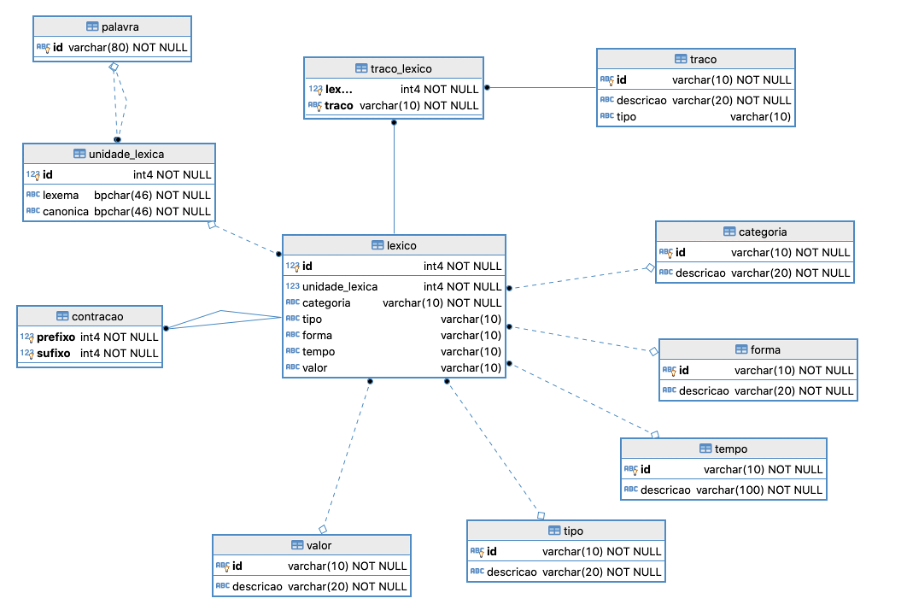
\includegraphics[width=\textwidth]{Fig2.png}
 \caption{Modelo entidade-relacionamento do Banco de Dados.}
 \label{fig2}
 \source{Autoria própria.}
\end{figure}

No processo de construção do Banco de Dados, foram atendidas algumas especificidades quanto à natureza do nosso léxico. Uma unidade do léxico como “casa”, por exemplo, pode pertencer a duas categorias gramaticais, verbo e substantivo. Caso seja verbo, a forma canônica corresponde ao verbo no infinitivo “casar”; caso seja substantivo, a forma canônica corresponde ao substantivo feminino “casa”. A duplicação dentro de uma base pode ser um desperdício de memória e tomar tempo maior para a consulta de dados. Para dar conta dessa ambiguidade, foram criadas três tabelas: Palavra, Unidade Léxica e Léxico. A estratégia de criar essas três tabelas permitiu que a unidade lexical “casa”, por exemplo, fosse armazenada apenas uma vez na tabela Palavra e que ela fosse só referenciada nas tabelas Unidade Léxica e Léxico (\Cref{fig2}) por meio do índice (id). Assim, na tabela Unidade Léxica, a palavra “casa” é armazenada como verbo e substantivo sem que se repita no banco.

Consideramos a palavra associada à sua forma canônica como uma unidade lexical que embasa a estrutura do nosso Banco de Dados, assim como ocorre no conjunto lexical do DELAF\_PB. Para as categorias de pessoa, gênero, grau e número, manteve-se o padrão linguístico de reuni-las dentro da tabela de traço semântico (Traço). Isso está de acordo também com o que propôs Bryce-Codd (1972 apud \cite[p. 75]{lake_concise_2013}) 
em sua “Quarta Forma normal” para padronização de dados. Essa solução permitiu contemplar a característica do nosso Banco de Dados, em que uma classe pode conter muitos traços e um traço semântico pode ser atribuído a várias classes, conforme \Cref{fig2}.

Finalmente, adotamos uma estratégia para dar conta de contrações, ou seja, de aglutinações de preposições e pronomes com outras palavras as quais geram um novo vocábulo, entradas que estão representadas no DELAF pela união de duas classes pela letra “X” (como em PREPXART para a unidade lexical “da”, preposição “de” mais artigo “a”). Como nem combinações, nem contrações envolvem diretamente categorias gramaticais e, por definição, têm independência em relação a elas, a estratégia consistiu em agrupá-las em uma nova entidade com cada entrada identificada pelo prefixo e sufixo correspondentes. Isso foi feito por meio da tabela Contração (\Cref{fig2}), que recebe o sufixo e o prefixo da tabela Léxico. As categorias utilizadas foram as seguintes: PROXPRO, contração de pronome com pronome, como “aqueloutra”, por exemplo; PREPXADV, contração de preposição mais advérbio, como “dali”; PREPXART, contração de preposição mais artigo, como nos casos de crase “à” e “do”, no sentido de posse, como em “carro do homem”; PREPXPRO, contração de preposição mais pronome, como “nalguma”, com sentido de “em alguma”; e PREXPREP, como em “dentre”.

O Banco de Dados povoado contém 860.778 palavras, 879.155 unidades léxicas e um total de 1.193.295 unidades léxicas classificadas (uma unidade léxica pode pertencer a mais de uma categoria lexical). A descrição de todas as categorias gramaticais encontra-se documentada em \textcite{pacheco_banco_2021}. 

\section{Aspectos técnicos e regras utilizadas na construção do \textit{Parser Parsero}, um algoritmo de Processamento de Linguagem Natural}\label{sec-formato}
O processador sintático Parsero foi desenvolvido em linguagem GO \cite{the_go_authors_golang_nodate} sob o padrão MVC (Modelo-Visão-Controlador), que é uma base comum para muitos modelos baseados em Web \cite[p. 108]{sommerville_engenharia_2011}(. O programa é uma API (Application Programming Interface) criada com a biblioteca Gorilla Mux \cite{the_gorilla_authors_gorilla_2021}. Esse padrão de projetos MVC tem três partes, assim utilizadas em nosso Parser: no Modelo, primeira parte, ficam as funções para consulta e inserção dos dados na base léxica, as quais foram descritas na seção anterior. A Visão, segunda parte, abriga um único endereço que, ao ser chamado, aciona o Controlador, terceira parte, em que estão abrigadas as instruções do algoritmo. O Controlador, então, executa as seguintes tarefas: recebe a sentença, consulta a base de dados e retorna as possibilidades de classificação para cada palavra. Depois disso, recebe esse resultado e percorre as regras de produção, as quais detalharemos nesta seção (\Cref{tbl2}), até encontrar uma válida para a sequência. No final, retorna um arquivo de texto com as unidades lexicais rotuladas de acordo com suas categorias, agrupadas em sintagmas e encapsuladas em formato (JSON) JavaScript Object Notation \cite{ecma-404_internacional_json_2017}.

O método escolhido para percorrer as regras foi a Análise Sintática Descendente Recursiva (ASDR) com derivação à esquerda \cite[p. 37]{thain_introduction_2020}. As regras de produção formam uma árvore que pode ser percorrida da raiz, a sentença, até as folhas, os núcleos funcionais. Nessa estrutura, os sintagmas são os ramos da árvore, e os nós que ficam localizados onde seriam as folhas são representados pelos núcleos sintáticos definidos nas regras (\Cref{tbl2}). A ASDR caminha pela árvore da raiz até as folhas sempre executando primeiro o nó à esquerda. Em nossa abordagem, ela recebe um vetor com as classes possíveis para cada palavra e, ao atingir uma folha da árvore, compara cada possibilidade de classificação com o núcleo funcional da regra vigente. O ciclo é repetido até não haver mais possibilidades. 

O algoritmo completo para um conjunto de regras de produção de tamanho $n$, em que cada possibilidade de produção é representada pelo símbolo $\beta_i$, é o seguinte:

\begin{algorithm}[H]
\SetAlgoLined
\BlankLine
\SetKwInOut{Input}{entrada}\SetKwInOut{Output}{retorno}
\Input{sentença}
\Output{regra válida}
\BlankLine

\SetKwFunction{FMain}{Principal}
\SetKwProg{Fn}{Função}{:}{fim} 
\Fn{\FMain{sentença}}{
    escolher uma produção $\alpha$ tal que $\alpha \rightarrow \beta_1 | \beta_2 | \ldots | \beta_n$
    
    \ParaCada{$i$ de 1 a $n$}{
       \uSe{$\beta_i$ é um não terminal NT}{invocar procedimento $\beta_i( )$}
       \uSenaoSe{($\beta_i$ é um terminal $\Sigma$) e ($\beta_i$ == símbolo atual)}{avance na sentença para o próximo símbolo}
       \Senao{\Retorna{regra inválida}}
       \Retorna{regra inválida}
       }
  }
\BlankLine
%\caption{aaaa}
\end{algorithm}

Como cada regra de produção pode evocar a si mesma a cada momento, o algoritmo tem natureza recursiva. Uma sentença é considerada inválida se não pode ser expressa por nenhuma das regras de produção estabelecidas e, se há um erro, ele é classificado em erro de léxico (quando não encontra palavra no Banco de Dados), erro sintático (sentenças agramaticais) ou erro interno (evento inesperado como queda da rede, problema de acesso ao Banco de Dados etc.). A interface gráfica final foi construída com a biblioteca \textit{React} em linguagem EcmaScript 6 \cite{ecma_internacional_ecmascriptlanguage_2015}.

Para a construção das regras de produção, utilizamos como base aquelas propostas por \textcite{othero_gramatica_2009}, que, por sua vez, seguem a Teoria X-Barra que é, no dizer de \textcite[p. 389-398]{chomsky__2014}, uma segunda fase, para além dos “primórdios da gramática da estrutura sintagmática” \textcite[p. 390]{chomsky__2014}. Um dos pontos destacados por Chomsky acerca dessa teoria é que 

\begin{quote}
    ao invés de aparecer como nas gramáticas de estrutura sintagmática tentando construir a estrutura de cima para baixo (‘\textit{top-down}’), aqui ela se move dos itens lexicais para cima. Assume que os itens lexicais já vêm colocados em um pequeno conjunto de categorias possíveis, em que cada item em cada categoria possui um conjunto de traços que na verdade dizem o que o item lexical relevante pode fazer em uma derivação/computação. Assim, na medida em que um item lexical se ‘projeta’ por meio da estrutura, ele carrega seus traços com ele, e estes determinam como eles podem se combinar, onde, e como eles irão ser lidos \cite[p. 392]{chomsky__2014}.
\end{quote}

Desse modo, é possível elaborar macrorregras gramaticais que prevejam estruturas como complementos e adjuntos, por exemplo. As regras são orientadas para conseguir representar estruturas sintáticas cujo núcleo exige ou aceita complementos e regras gramaticais que possibilitem analisar sintagmas cujo núcleo não aceita ou não exige complementos. Empregando os conceitos da Teoria X-Barra, nosso \textit{Parser} consegue lidar com sentenças como em (9) “A casa verde foi ocupada” e (10) “A casa de Maria foi ocupada”, conforme \Cref{fig3} e \Cref{fig4} respectivamente.



O diagrama da \Cref{fig3} representa um adjunto adnominal, e o da \Cref{fig4} um complemento nominal. Não contemplamos, neste projeto, a distinção entre complementos e adjuntos, uma vez que os Sintagmas Preposicionais podem assumir tanto as funções de complemento nominal quanto de adjunto adnominal e que, para distinguir essas funções, teríamos de recorrer a critérios de ordem “predominantemente semântico-pragmática” \cite[p. 25]{souza_e_silva_linguistica_2011}.

Em \textcite[p. 142]{othero_gramatica_2009}, as regras de produção são formadas por um núcleo funcional único, que pode ser: Determinante (D), Substantivo (N), Verbo (V), Adjetivo (A), Advérbio (Adv), Preposição (P), Quantificador (Q), Numeral (Num). Também pode ser formado por um sintagma ou por um nó X-Barra, que pode conter ou não um complemento, por isso a notação (’) aparece ao lado dele. 

Nas regras definidas por \textcite[p. 142]{othero_gramatica_2009}\footnote{Optamos por adaptar a terminologia das regras de \textcite{othero_gramatica_2009}, que usa a terminologia inglesa \textit{Phrasal}. Preferimos, como estamos trabalhando com o Português Brasileiro, a expressão Sintagma. Desse modo, usaremos SN, SV, SA, Sadv, SP e assim por diante, como Sintagma Nominal, Sintagma Verbal, Sintagma Adjetival, Sintagma Adverbial, Sintagma Preposicionado etc.}, cada um dos sintagmas é composto por um núcleo funcional que representa o símbolo central do sintagma. Foram definidos os seguintes sintagmas: a) Nominais (SN): têm como núcleo os Substantivos (N); b) Determinantes (SD): podem conter como núcleo Artigos, Pronomes Demonstrativos, Pronomes Pessoais ou estarem ocultos na sentença. São representados como determinantes (D); c) Numerais (SNum): têm como núcleo os Numerais (Num); d) Possessivos (SPoss): têm como núcleo os Pronomes Possessivos (Poss); e) Quantificadores (SQ): têm como núcleo os quantificadores como algum, todos, cada, nenhum; f) Adjetivais (SA): têm como núcleo os Adjetivos (A); g) Adverbiais (SAdv): têm como núcleo os Advérbios (Adv); e h) Verbais (SV): têm como núcleo os Verbos (V).

Além desses sintagmas, utilizaremos, ainda, dois outros sintagmas para lidar com sentenças complexas. O primeiro, o Sintagma Flexional (SI, do \textit{Inglês Inflectional Phrase}), dá conta das sentenças que contêm mais de um verbo em sua estrutura. Quando isso ocorre, esses dois verbos são genericamente entendidos como locuções verbais pelo nosso Parser, independentemente de serem essas locuções constituídas ou não por um verbo principal, que não se flexiona, mais um auxiliar, como em (11) “Maria vai sair” (\Cref{fig5}), ou por dois verbos principais, que são passíveis de serem flexionados, como em (12) “Maria acordou chorando” (\Cref{fig6}). Para uma discussão mais profunda sobre locuções verbais, encaminhamos o leitor para \textcite[p. 126-131]{othero_gramatica_2009}.


Além disso, recorremos à solução de \textcite{othero_gramatica_2009} para tratar estruturas com orações subordinadas conectadas por conjunções, acrescentando o SC (Sintagma Complementizador), conforme descrito pelo autor:

\begin{quote}
    A posição de núcleo do CP [SC em nosso Parser] será ocupada por \textbf{que}, \textbf{se} ou \textbf{quando} (como em João sabe se a Maria lê bastante; João sabe quando a Maria chegou). Com essas mesmas regras, podemos analisar também frases que contenham uma estrutura verbo auxiliar + verbo principal dentro do IP complemento (A Maria disse que iria chegar mais tarde) \cite[p. 139, grifos do autor]{othero_gramatica_2009}.
\end{quote}

Nosso \textit{Parser} executou corretamente essas estruturas, conforme exemplo da \Cref{fig7}, (13) “João sabe se a Maria lê bastante”.



Além disso, o Sintagma Complementizador, que denominamos SC em nosso trabalho, permite que se processem frases com estruturas recursivas como em (14) “A Maria disse que João falou que estava com fome” (\Cref{fig8}).



Quanto à ordem de processamento das regras, nosso Parser adotou o método de processar primeiro as mais complexas, em que há mais do que um núcleo funcional na regra. Por exemplo, em (15) “O carro azul”, opta-se primeiro pelo processamento das regras em que o substantivo (N) é precedido ou sucedido de um adjetivo (A) (regras N’ → N’ SA e N’ → SA N’), e somente se essas regras não são válidas parte-se para a regra mais simples em que só há um substantivo (N’ → N). Não fosse desse modo, em estruturas como (15), o processamento terminaria antes que todas as palavras pudessem ser avaliadas, porque a regra anterior (N’ → N) já seria executada com sucesso, o adjetivo seria descartado e seguir-se-ia para o restante da sentença. Com essa mudança foi necessário também adaptar regras que poderiam resultar em recursões infinitas à esquerda, conforme exemplo na \Cref{tbl1}.

\begin{table}[htbp]
\caption{Exemplo de eliminação da recursão à esquerda.}
\label{tbl1}
\centering
\begin{tabular}{ll}
\toprule
\textbf{Antes} & \textbf{Depois} \\ 
\midrule
SN → N’  & SN → N’  \\ 
N’ → N’ SP       & N’ → N N’’   \\ 
N’ → N      & N’’ → SP N’’   \\
& N’’ → nulo   \\
\bottomrule
\end{tabular}
\source{Autoria própria.}
\end{table}

Na \Cref{tbl1}, o Sintagma Nominal apresentava recursividade infinita à esquerda na regra (N’ → N’ SP), que foi substituída pelas regras (N’ → N N’’) e (N’’ → SP N’’). O símbolo N’’ foi criado, podendo não conter valor nenhum. Quando aplicado a todas as regras, esse raciocínio levou à formação de novos símbolos X-Barra (\Cref{tbl2}). Em alguns casos, o elemento nulo foi explicitamente usado para identificar a possibilidade de ocultar o elemento. 

Esse raciocínio segue o método da fatoração à esquerda, que consiste na reescrita de uma regra para adiar seu processamento até que ele seja possível \cite[p. 41]{thain_introduction_2020}. Por exemplo, pelas regras de \textcite{othero_gramatica_2009}, a frase (16) “O jogador de futebol caiu” geraria um ciclo infinito em nosso algoritmo ao tentar classificar a palavra “jogador”, porque o nó N’ retornaria a si mesmo (na sequência N’ → N’) se não fossem especificadas outras regras para que o processador não percorra novamente regras pelas quais já passou. Pelas novas regras, ao chegar ao nó N’, é obrigatória a existência de um substantivo (N’ → N N’’). Se não for possível classificar a palavra como substantivo, o algoritmo não prossegue. Feitas essas adaptações, a Gramática do \textit{Parsero} ficou composta pelas regras apresentadas na \Cref{tbl2}.

\begin{table}[htbp]
\caption{Regras de Produção para o \textit{Parser Parsero}.}
\label{tbl2}
\centering
\begin{tabular}{| l | l | l |}
\hline
Sintagma Inflexional & Sintagma Numeral & Sintagma Preposicional \\ 
SI → SD I' & SNum → Num & SP → P' \\
SI → I' & SNum → Num SP; & P' → SAdv P' \\
I' → I'' SV & &  P' → P SD \\
I'' → I I'' & Sintagma Possesivo & P' → P SAdv \\
I'' → SD I'' & SPoss → Poss SN & P' → P SC \\
I'' → nulo & SPoss → SN Poss & P' → P SP \\
 & SPoss → Poss SNum; & P' → P; \\
Sintagma Complementizador & Sintagma Quantificador & Sintagma Adverbial \\
SC → C SI; & SQ → Q SD & AdvP → Adv' \\
Sintagma Determinante &  SQ → Q SP & Adv' → Adv SP \\
SD → D SN & SQ → SD Q; & Adv' → Adv Adv'' \\
SD → D SPoss &   & Adv'' → Adv' Adv'' \\
SD → D SNum & Sintagma Adjetival & Adv'' → nulo; \\
SD → SN & SA → A' & Sintagma Verbal \\
SD → SPoss & A' → SAdv A' & SV → V' \\
SD → SNum & A' → A SP & V' → SAdv V' \\
SD → D & A' → A SC & V' → V SD \\
 & A' → A A''& V' → V SP \\ 
Sintagma Nominal & A'' → SAdv A'' & V' → V SC \\ 
SN → N' & A'' → SP A'' & V' → V SA \\ 
N' → N SP & A'' → nulo; & V' → V SAdv \\ 
N' → N SC &  & V' → V SI \\ 
N' → N N'' &  & V' → V V'' \\ 
N' → AP N' &  & V'' → SAdv V'' \\ 
N'' → SC N'' &  & V'' → PP V'' \\ 
N'' → SP N'' &  & V'' → nulo; \\ 
N'' → SA N'' &  & \\ 
N'' → nulo; &  &  \\ 
\hline
\end{tabular}
\source{Adaptação de \textcite[p. 142]{othero_gramatica_2009}.}
\end{table}

Nos casos em que o adjetivo precede o substantivo e que esse adjetivo também pode ser um substantivo, como em (17) “O pobre homem de Roma morreu”, adotou-se a regra de prioridade para que as palavras que vêm em primeiro lugar sejam categorizadas pelo Parser como substantivos e as que vêm em segundo como adjetivos, pois essa é a forma mais comum no Português Brasileiro, que admite tanto as formas “pobre homem” como “homem pobre”, diferente do Inglês, por exemplo, que admite apenas “poor man” . As \Cref{fig3}, \Cref{fig4}, \Cref{fig5}, \Cref{fig6}, \Cref{fig7} e \Cref{fig8}, apresentadas neste trabalho, são resultados gerados pelo aplicativo.

\section{Considerações finais}\label{sec-modelo}
Este artigo apresentou a construção de um Parser Sintático para o Português Brasileiro, que utilizou o recurso disponível na Internet, o Dicionário DELAF\_PB \cite{muniz_construcao_2004} e as regras propostas por \textcite[p. 142]{othero_gramatica_2009}, estas, por sua vez, baseadas no conceito de Gramática Gerativa, de \textcite{chomsky_estruturas_2015}, e expandidas pela Teoria X-Barra \cite{chomsky__2014,othero_gramatica_2009}. 

A partir das regras, empreendemos um intenso processo de refatoração para adaptá-las ao algoritmo utilizado (Algoritmo Descendente Recursivo), o que nos levou à criação de novas regras que eliminaram os ciclos recursivos à esquerda, facilitando o processamento. 

A base léxica no formato DELA foi adaptada para o formato SQL e disponibilizada em código aberto. O projeto do Banco de Dados respeita o formalismo de Bryce-Codd (1972 apud \cite[p. 75]{lake_concise_2013}),  
e evitou duplicações para poupar memória de processamento. A estrutura proposta permitiu também que novas palavras pudessem ser inseridas sem classificação, o que priorizou a expansão do léxico. Essa estrutura deixa aberta a possibilidade de que posteriormente as palavras possam ser classificadas manualmente por usuários ou por métodos matemáticos apreendidos a partir da base já existente. 

A tela de interação com o usuário foi desenvolvida em linguagem GO, sob o padrão MVC, Model (modelo) View (visão) e Controller (Controle), padrão que facilita a troca de informações entre a interface do usuário e os dados no banco, fazendo com que as respostas sejam mais rápidas e dinâmicas. Para processar as sentenças simples e compostas do Português Brasileiro, sem uso de pontuação, foi gerada uma API que as analisa e exibe a árvore sintática por meio de uma interface gráfica.

Além de ter propiciado reflexões sobre as potencialidades da Gramática Gerativa para o desenvolvimento de Processadores de Linguagem Natural, notadamente para atender às sofisticadas construções sintáticas do Português Brasileiro, este trabalho também constituiu uma oportunidade de pesquisa interdisciplinar que buscou aproximar as ciências da linguagem e as ciências da computação. Além disso, disponibilizar os resultados, tanto a base de dados quanto o algoritmo, é um estímulo para que outros pesquisadores possam aperfeiçoar ou possam criar outros processadores sintáticos que serão a base para sistemas inteligentes os quais possam interagir com escritores ou falantes do Português.

\printbibliography\label{sec-bib}
% if the text is not in Portuguese, it might be necessary to use the code below instead to print the correct ABNT abbreviations [s.n.], [s.l.]
%\begin{portuguese}
%\printbibliography[title={Bibliography}]
%\end{portuguese}


%full list: conceptualization,datacuration,formalanalysis,funding,investigation,methodology,projadm,resources,software,supervision,validation,visualization,writing,review
\begin{contributors}[sec-contributors]
\authorcontribution{Manoel Francisco Guaranha}[conceptualization,methodology,validation,supervision,review]
\authorcontribution{Willian Emerson Afonso Pacheco}[methodology,software,writing]
\end{contributors}

\newpage
\appendix
\section{Apêndice}\label{sec-apendice}
\begin{figure}[h]
 \centering
 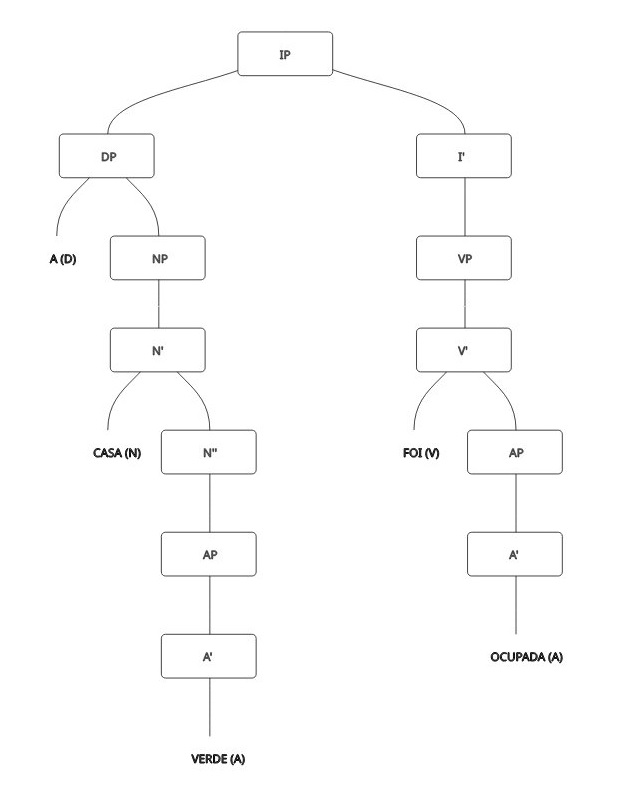
\includegraphics[width=0.9\textwidth,height=0.8\textheight,keepaspectratio]{Fig3.png}
 \caption{Diagrama arbóreo de Sintagmas Nominais – Teoria X-Barra – sentença: “A casa verde foi ocupada” (9).}
 \label{fig3}
 \source{Autoria própria. Interface gráfica do \textit{Parsero} 1.0.}
\end{figure}

\begin{figure}[p]
 \centering
 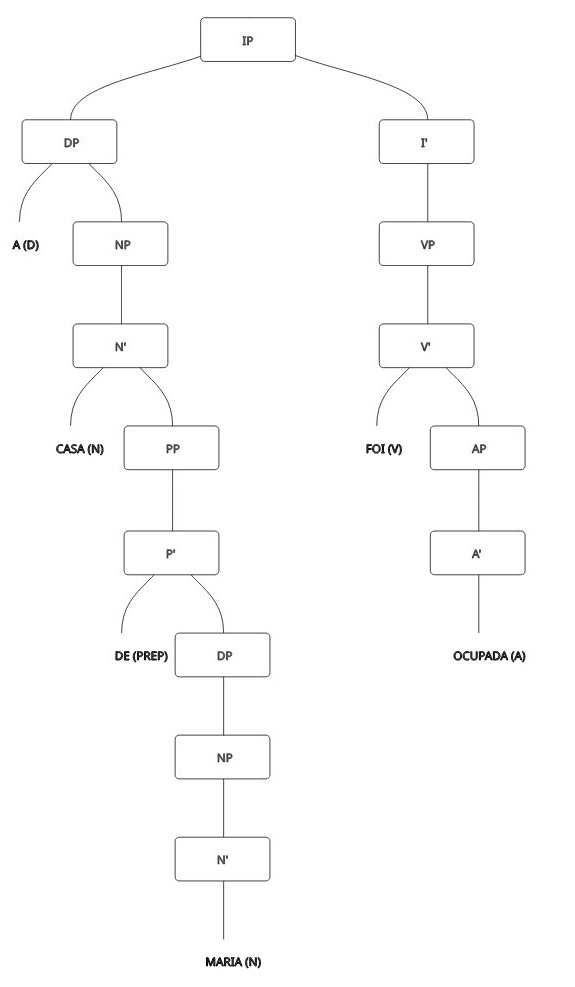
\includegraphics[width=\textwidth,height=0.85\textheight,keepaspectratio]{Fig4.png}
 \caption{Diagrama arbóreo de Sintagmas Nominais – Teoria X-Barra – sentença: “A casa de Maria foi ocupada” (10).}
 \label{fig4}
 \source{Autoria própria. Interface gráfica do \textit{Parsero} 1.0.}
\end{figure}

\begin{figure}[p]
 \centering
 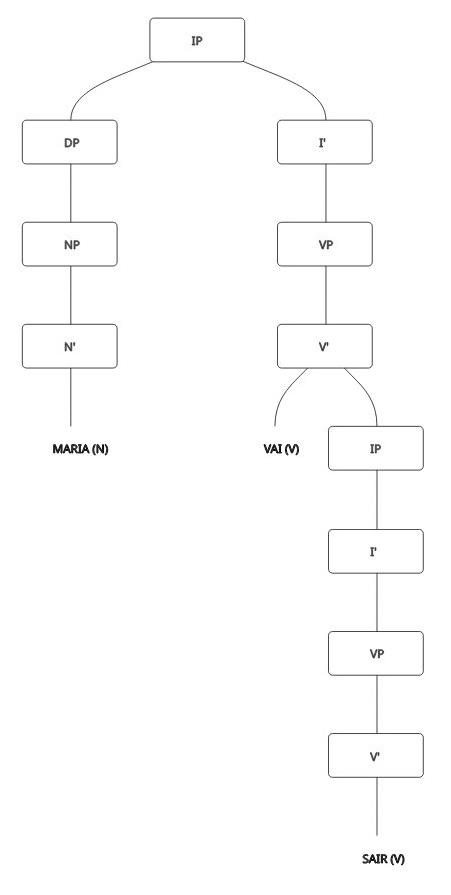
\includegraphics[width=\textwidth,height=0.85\textheight,keepaspectratio]{Fig5.png}
 \caption{Sentença com verbo auxiliar: “Maria vai sair” (11).}
 \label{fig5}
 \source{Autoria própria. Interface gráfica do \textit{Parsero} 1.0.}
\end{figure}

\begin{figure}[p]
 \centering
 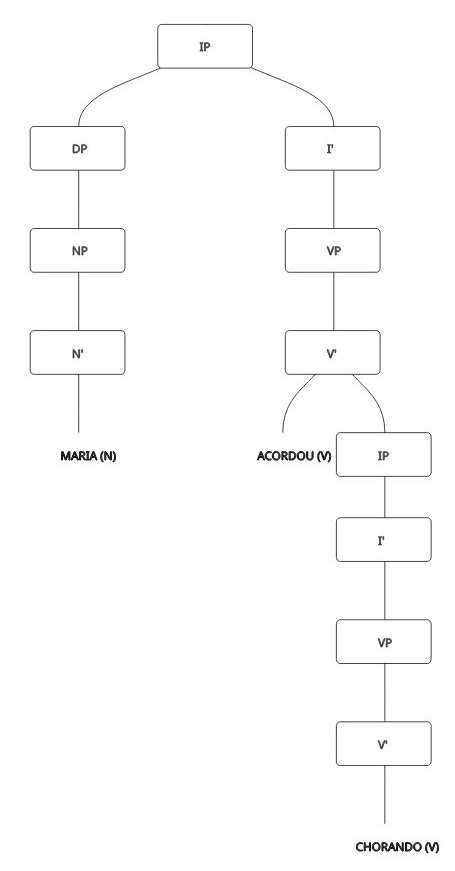
\includegraphics[width=\textwidth,height=0.85\textheight,keepaspectratio]{Fig6.png}
 \caption{Sentença com dois verbos principais: “Maria acordou chorando” (12).}
 \label{fig6}
 \source{Autoria própria. Interface gráfica do \textit{Parsero} 1.0.}
\end{figure}

\begin{figure}[p]
 \centering
 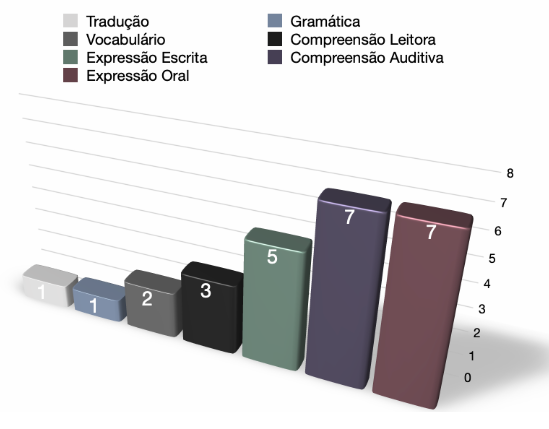
\includegraphics[width=\textwidth,height=0.85\textheight,keepaspectratio]{fig7.png}
 \caption{Exemplo de sentença com Sintagma Complementizador – “João sabe se a Maria lê bastante” (13).}
 \label{fig7}
 \source{Autoria própria. Interface gráfica do \textit{Parsero} 1.0.}
\end{figure}

\begin{figure}[p]
 \centering
 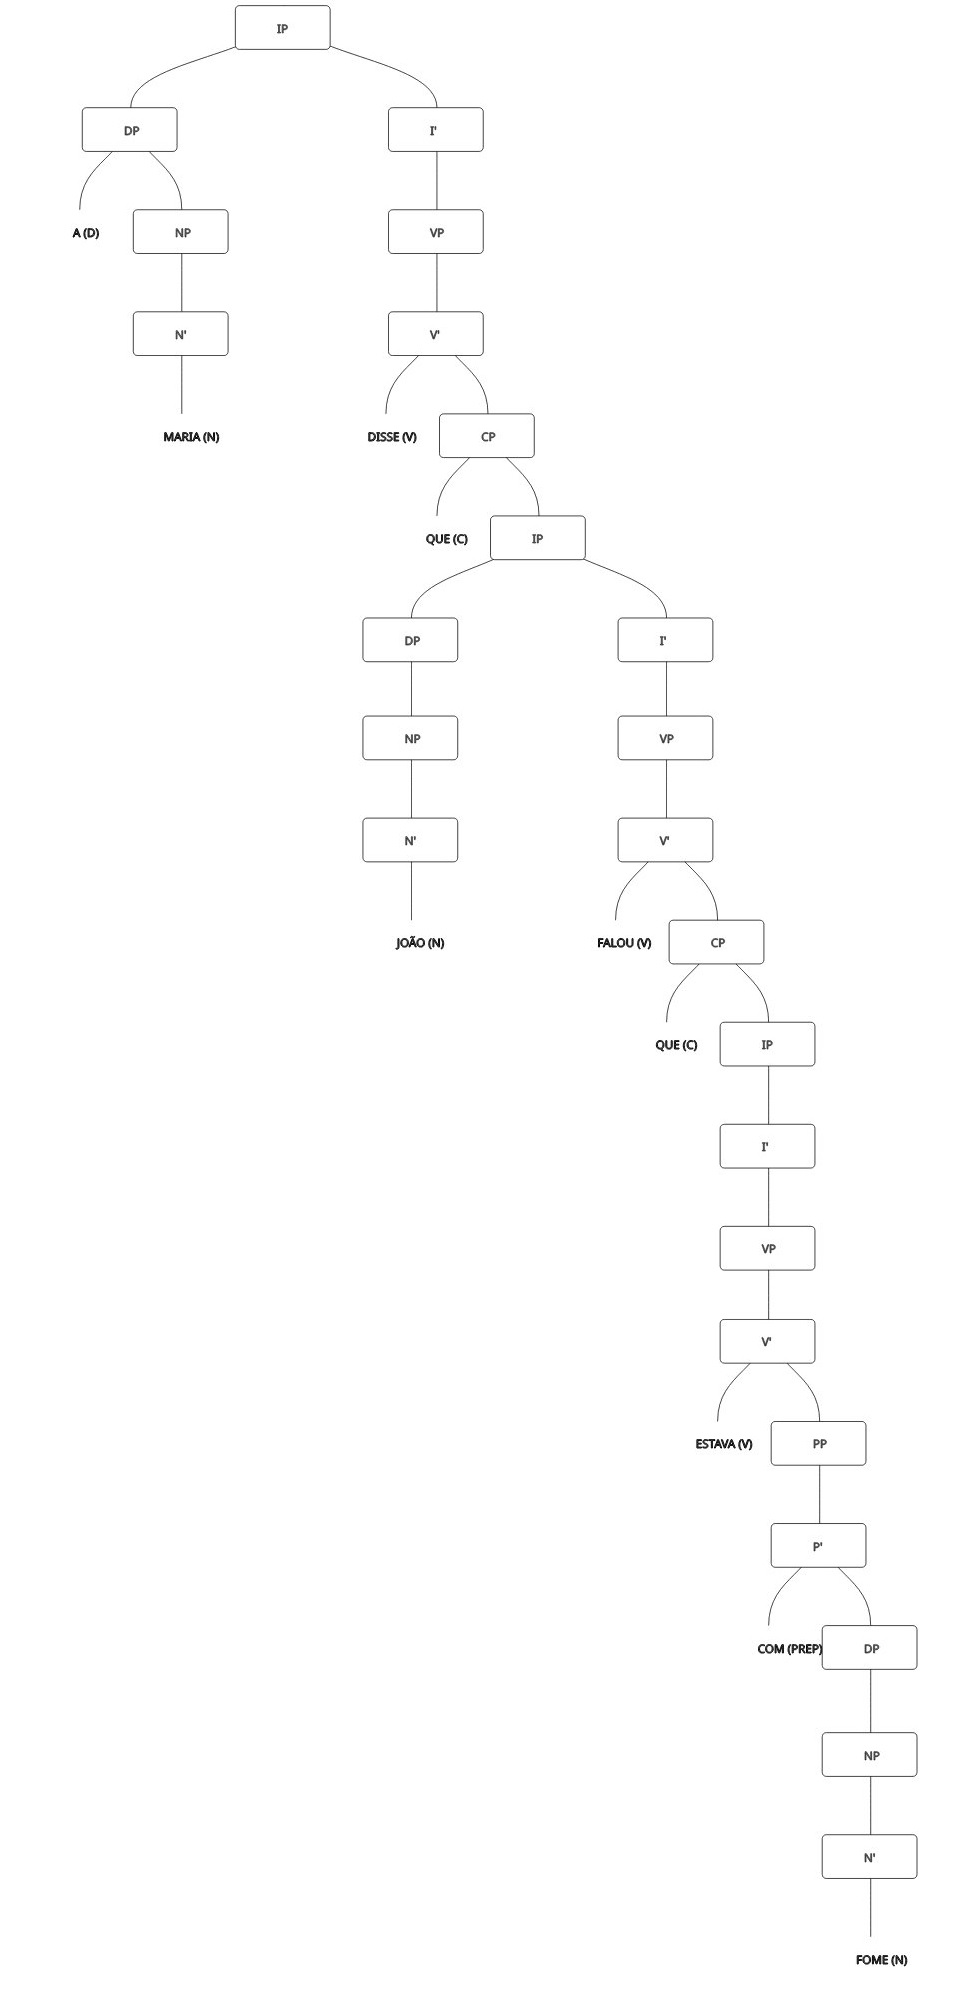
\includegraphics[width=\textwidth,height=0.85\textheight,keepaspectratio]{Fig8.png}
 \caption{Exemplo de sentença com estrutura recursiva – sentença: “A Maria disse que João falou que estava com fome” (14).}
 \label{fig8}
 \source{Autoria própria. Interface gráfica do \textit{Parsero} 1.0.}
\end{figure}

\end{document}